\chapter{Physical Simulations}
Modeling the world around us is a longstanding problem of science. For many
physical processes, model equations exist, describing how a given system evolves
through time. From weather and climate forecasts (\cite{stocker2014climate})
over quantum physics (\cite{QuantumSim}), to the control of plasma fusion
(\cite{PlasmaControl}), or optimizing the shape of
vehicles (\cite{OptimizationCFD}), it has become an integral part of engineering
applications to use numerical methods to derive solutions from model equations.

In this section, we build up an understanding of modeling physical phenomena
with \acfp{PDE}. We also introduce the notion of \acf{DP} after a brief
introduction to classical numerical methods.

\section{Partial Differential Equations}
\acp{PDE} are the most fundamental description of evolving systems from quantum
mechanics to turbulent flows. \acp{PDE} are equations relating the partial
derivatives of some unknown function. For a physical system $\vb{u}(\vb{x},t)$,
the governing \ac{PDE} can be written as

\begin{equation}
\label{eq:pde}
\pdv{\vb{u}}{t} = \mathcal{P}\left(\vb{u}, \pdv{\vb{u}}{\vb{x}},
\pdv[2]{\vb{u}}{\vb{x}},\dots,\vb{y}(t)\right),
\end{equation}
where $\mathcal{P}$ models the physical behavior of the system, and $\vb{y}(t)$
denotes an (optional) external force factor. 

\todo{Should we give example(s) of a PDE here? (e.g. Dirichlet boundary
condition, Navier-Stokes, Burger's Equation, or anything else?)}

\subsection{Numerical Methods}
Analytic solutions (i.e. closed-form expressions) can be found usually only for
very simple \acfp{PDE}. 

\todo{How much does it makes sense to write about these?}
\todo{
  Numerical Integration:
  \begin{itemize}
    \item Euler Step
    \item Midpoint
    \item RK4
  \end{itemize}
  Finite Differences:
  \begin{itemize}
    \item Replace domain by a finite number of discrete points.
    \item These points are typically located on Eulerian grid.
    \item Discretization: Central difference gives approximation of derivatives.
  \end{itemize}
  $\left( \pdv{q}{x}\right)_i = \frac{q_{i+1} - q_{i-1}}{2\Delta x}$
  ($\pdv{q}{x}$ at grid point $i$) $\rightarrow$ staggered grid: 
  $\left( \pdv{q}{x}\right)_i = \frac{q_{i+1/2} - q_{i-1/2}}{2\Delta x}$
    Finite Elements: (Is the Eigenfluid simulation a Finite Elements method?)
  \begin{itemize}
    \item Replace infinite dimensional solution space by a finite dimensional
      solution space
    \item Function space is constructed by decomposing domain into a set of
      "finite elements" and defining interpolation functions for them
  \end{itemize}
  $\to$ Finite number of unknowns
}

\section{Differentiable Physics}
Given $\vb{u}(\vb{x}, t)$, described by a \ac{PDE} as in Equation~\eqref{eq:pde}, a regular
solver can move the system forward in time via Euler steps:

$$\vb{u}(\vb{x},t) = \text{Solver}\left[ \vb{u}(t_i), \vb{y}(t_i) = 
  \vb{u}(t_i) + \Delta t \cdot \mathcal{P} \left( 
    \vb{u}(t_i), \dots, \vb{y}(t_i)
  \right)
\right],$$

computing a solution trajectory $\vb{u}(t)$, that approximates a solution to the
\ac{PDE}. Although this computation is differentiable, it is not well-suited to
solve optimization problems, since gradients can only be approximated by finite
differencing, and (especially for high-dimensional or continuous systems), this
method would become computationally expensive, because a full trajectory needs
to be computed for each optimizable parameter.

\cite{holl2019pdecontrol} address this issue via the use of differentiable
solvers, solving the adjoint problem \todo{cite?} via analytic derivatives.
Differentiable solvers can efficiently compute the derivatives with respect to
any of the inputs $\pdv*{\vb{u}(t_{i+1})}{\vb{u}(t_i)}$ and
$\pdv*{\vb{u}(t_{i+1})}{\vb{y}(t_i)}$

\todo{
\begin{itemize}
  \item Example of a differentiable language built for CG: DiffTaichi
    introduced by \cite{difftaichi}
  \item todo link phiflow, we are using that for our implementation
\end{itemize}
}


\todo{Write short intro on optimization?}

For a basic comparison of the characteristics of supervised and differentiable
physics approaches, see Figure~\ref{fig:learning-to-throw}.

\section{Loss Functions}
\todo{Write about inductive physical bias}
\todo{Observation loss at end step should match target observation.
  Give only a high-level overview here? (And hatch it out more in the problem
  statement part later on?)
}

\begin{figure}
  \centering
  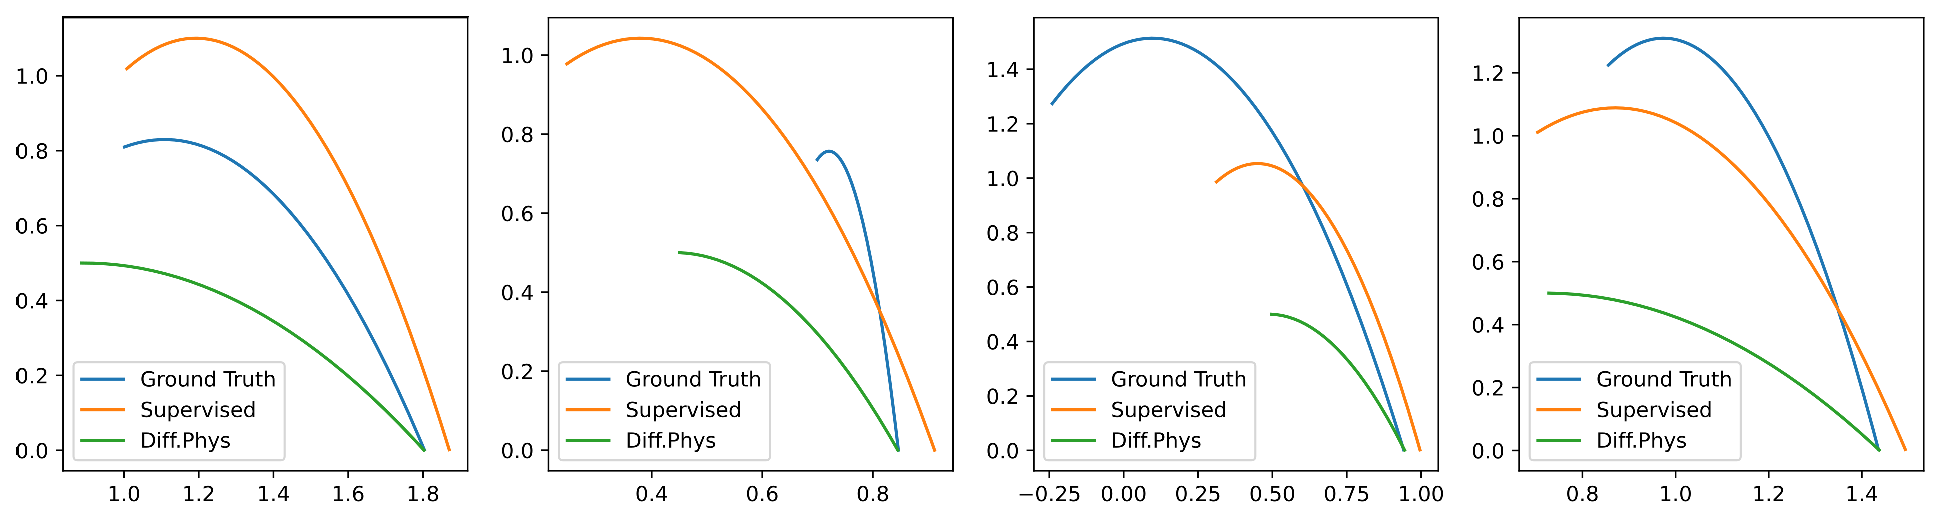
\includegraphics[width=0.8\textwidth]{figures/throwing_results}
  \caption{Learning to throw. 
    An example, showcasing an important difference between supervised and
    differentiable physics approaches. Both the supervised and the
    differentiable physics network approximate the function
    $f^{-1}(\vb{x_{final}}): \mathbb{R} \mapsto \mathbb{R}^4$, which is the
    inverse of the function $f(\vb{x}, \vb{y}, \vb{v}, \vb{\alpha})$, mapping
    the final position $\vb{x_{final}}$ of an object being thrown from position
    $(\vb{x}, \vb{y})$, with velocity $\vb{v}$ and angle $\vb{\alpha}$. The same
    network architecture is used, with the weights initialized to the same
    initial values. Both networks have seen the same number of training
    examples, and are using an $L_2$ norm between the point of impact resulting
    from the predicted initial values and the intended position. It is evident
    that the DP network is able to get orders of magnitude closer than the
    supervised network, which has no knowledge of the underlying physical
    system, and it's best guess is to interpolate between the closest data it
    has seen during training, which results in a coarse approximation. Also, as
    the result space to this problem is not unimodal (e.g. it has multiple
    possible right answers), the supervised model is further thrown off, and
    will give values in-between. This means that even if we increase the
    training data, our supervised model can never learn this problem properly.
    \todo{Should this be shorter?}
    \todo{How to link to this source:
      \url{https://tum-pbs.github.io/PhiFlow/Learn_to_Throw_Tutorial.html}?
      (It's one of the demos from phiflow)}
    }   
    \label{fig:learning-to-throw}
\end{figure}
